\documentclass[../sherrill-Mix_thesis.tex]{subfiles}
\begin{document}
\graphicspath{{im/}{pacBio/im/}}

\chapter{Dynamic regulation of HIV-1 mRNA populations analyzed by single-molecule enrichment and long-read sequencing}
\label{chapPacBio}

\section{Abstract}
Alternative RNA splicing greatly expands the repertoire of proteins encoded by genomes. Next-generation sequencing (NGS) is attractive for studying alternative splicing because of the efficiency and low cost per base, but short reads typical of NGS only report mRNA fragments containing one or few splice junctions. Here, we used single-molecule amplification and long-read sequencing to study the HIV-1 provirus, which is only 9700 bp in length, but encodes nine major proteins via alternative splicing. Our data showed that the clinical isolate \hivEight{} produces at least 109 different spliced RNAs, including a previously unappreciated $\approximately{}1$ kb class of messages, two of which encode new proteins. HIV-1 message populations differed between cell types, longitudinally during infection, and among T cells from different human donors. These findings open a new window on a little studied aspect of HIV-1 replication, suggest therapeutic opportunities and provide advanced tools for the study of alternative splicing. 

\section{Introduction}
Alternative splicing greatly expands the information content of genomes by producing multiple mRNAs from individual transcription units. Approximately 95\% of human genes with multiple exons encode RNA transcripts that are alternatively spliced, and mutations that affect alternative splicing are associated with diseases ranging from cystic fibrosis to chronic lymphoproliferative leukemia \citep{Pan2008,Wang2008,Pagani2005,Wang2007,Wang2011}. Work to decipher an RNA `splicing code' has revealed that multiple interactions between trans-acting factors and RNA elements determine splicing patterns, though regulation is little understood for most genes \citep{Barash2010}.

The integrated HIV-1 provirus is $\approximately{}9700$ bp in length and has a single transcription start site, but according to the published literature yields at least 47 different mRNAs encoding 9 proteins or polyproteins, making HIV an attractive model for studies of alternative splicing \citep{Purcell1993}. HIV mRNAs fall into three classes: the unspliced RNA genome, which encodes Gag/Gag-Pol; partially spliced transcripts, $\approximately{}4$ kb in length, encoding Vif, Vpr, a one-exon version of Tat, and Env/Vpu; and completely spliced mRNAs of roughly 2 kb encoding Tat, Rev and Nef (Figure \ref{figDonorAccept}A). Additional rare `cryptic' splice donors (\fivePrime{} splice sites) and acceptors (\threePrime{} splice sites) contribute even more mRNAs \citep{Benko1990,Carrera2010,Luetzelberger2006,Salfeld1990,Schwartz1990,Smith1992}. A complex array of positive and negative cis-acting elements surrounding each splice site regulates the relative abundance of the HIV-1 mRNAs, and disrupting the balance of message ratios impairs viral replication in several models \citep{Stoltzfus2009,Bakkour2007,Brass2008,Jablonski2009,Konig2008,Tranell2011,Zhou2008,Zhu2011}. Studies have suggested strain-specific splicing patterns may exist \citep{Purcell1993,Saltarelli1996,Delgado2012}. However, detailed studies of complete message populations have not been reported for clinical isolates of HIV-1. 

\begin{figure}
	\centering
	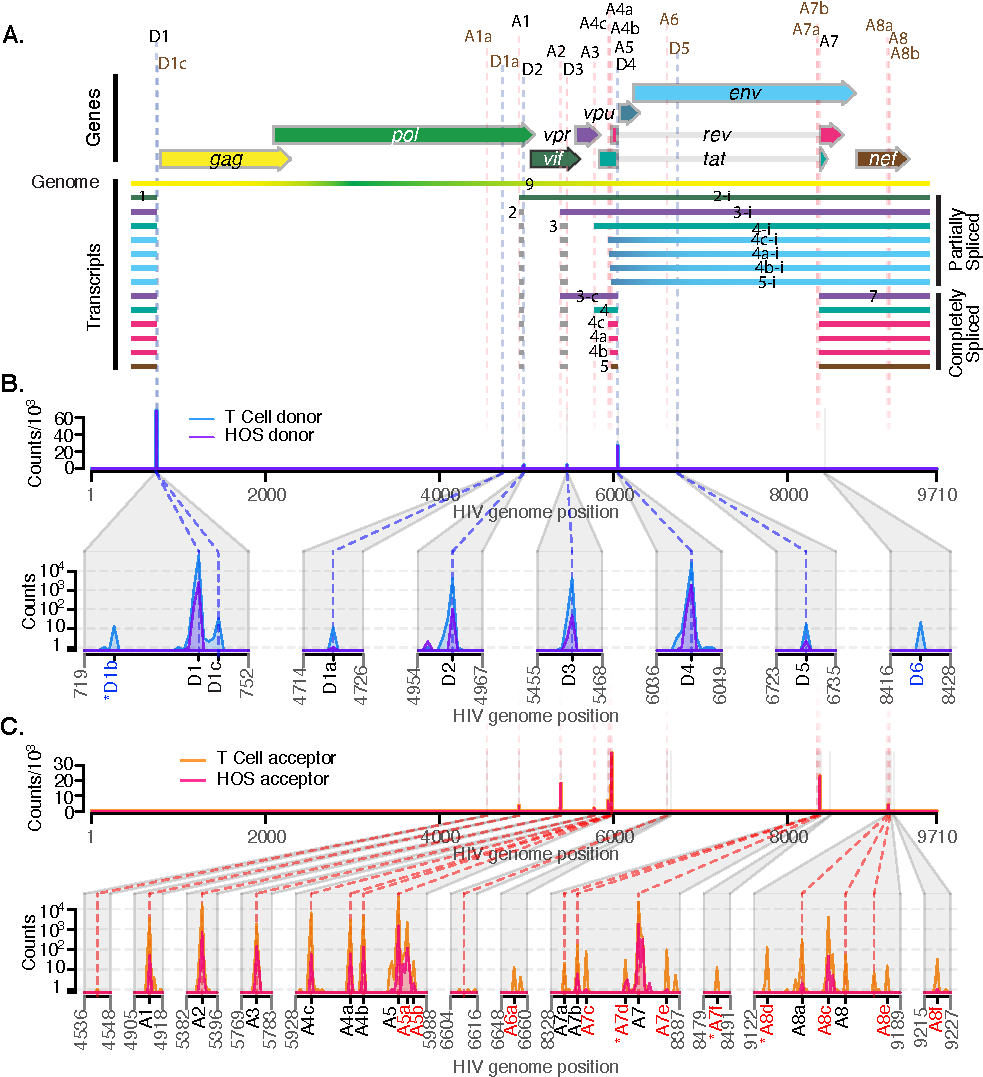
\includegraphics[width=.92\textwidth]{1.pdf}
	\caption[Mapping the splice donors and acceptors of \hivEight{}]{Mapping the splice donors and acceptors of \hivEight{}. PacBio sequence reads of \hivEight{} cDNA from infected HOS-CD4-CCR5 (HOS) and \cdFour{} T cells were aligned to the \hivEight{} genome shown in (A). Exons of the conserved HIV-1 transcripts are colored according to the encoded gene. Conserved (black) and published cryptic (brown) splice donors (`D') and acceptors (`A') are shown. Gaps in HIV-1 sequence alignments with at least one end located at a published or verified splice donor or acceptor were defined as introns. For each base of the \hivEight{} genome, the number of sequence reads in which that base occurred at the \fivePrime{}-end (B) or \threePrime{}-end (C) of an intron is plotted for each cell type. Putative splice donors and acceptors were defined as loci that were found in at least 10 reads at the \fivePrime{}- and \threePrime{}-ends of introns in sequence alignments from T-cell infections. Regions containing splice sites are enlarged for clarity. Asterisks indicate putative splice sites that are adjacent to dinucleotides other than the consensus GT and AG.}
	\label{figDonorAccept}
\end{figure}

Several groups have demonstrated tissue- and differentiation-specific splicing of cellular genes \citep{Wang2008,Grabowski2011,Llorian2011}. Importantly for HIV, these include changes during T-cell activation \citep{Ip2007,Topp2008}, raising the question of how cell-specific splicing affects HIV replication. While most studies of HIV-1 splicing have been conducted in cell lines using lab-adapted viral strains, limited works in PBMCs from infected patients, monocytes and macrophages have suggested that differences may indeed exist in relevant cell types \citep{Carrera2010,Saltarelli1996,Sonza2002,Dowling2008}. Moreover, human splicing patterns differ between individuals, but such polymorphisms have not been investigated in the context of HIV infection \citep{Hull2007,Kwan2007}.

Here, we use deep sequencing to comprehensively characterize the transcriptome of an early passage clinical isolate, \hivEight{} \citep{Collman1992}, in primary \cdFour{} T cells from seven human donors and in the human osteosarcoma (HOS) cell line. Many deep sequencing techniques provide short reads, which rarely query more than a single exon-exon junction. To distinguish the full structure of HIV-1 mRNAs, which can contain several splice junctions, we used Pacific Biosciences (PacBio) sequencing technology, which yields read lengths up to 10 kb \citep{Eid2009}. We used RainDance Technologies single-molecule PCR enrichment to preserve ratios of RNAs during preparation of sequencing templates. We identified previously published and novel HIV-1 transcripts and determined that \hivEight{} encodes a minimum of 109 different splice forms. These included a new size class of transcripts, some of which contain novel open reading frames (ORFs) that encode new proteins. We also found significant variation between cell types, over time during infection of HOS cells and among individuals. These data reveal unanticipated complexity and dynamics in HIV-1 message populations, begin to clarify a little studied dimension of HIV-1 replication and suggest possible targets for therapeutic interventions. 

\section{Materials and methods}
\subsection{Cell culture and viral infections}
\hivEight{} was generated by transfection and subsequent expansion in SupT1 cells. Primary T cells were isolated by the University of Pennsylvania Center for AIDS Research Immunology core and confirmed to be homozygous for the wild-type CCR5 allele as shown in Supplementary Table S1 and described in Supplementary Methods. HOS-CD4-CCR5 cells \citep{Deng1996,Landau1992} were obtained through the AIDS Research and Reference Reagent Program, Division of AIDS, NIAID, NIH from Dr Nathaniel Landau. Single round infections in T cells and HOS-CD4-CCR5 cells were performed using standard methods (see Supplementary Methods). 

\subsection{RNA and reverse transcription}
Total cellular RNA was purified using the Illustra RNA kit (GE Life Sciences, Fairfield, CT, USA) from $5 \times 10^6$ cells per infection. Viral cDNA was made using a reverse transcription primer complementary to a sequence in U3 (RTprime, Supplementary Table S2). We used Superscript III reverse transcriptase (Invitrogen) in the presence of RNaseOUT (Invitrogen) to conduct first-strand cDNA synthesis from equal amounts of total cellular RNA from each HOS-CD4-CCR5 time point (15.2 \ug{}) and from each T-cell infection (3 \ug{}) according to the manufacturer's instructions for gene-specific priming of long cDNAs, and then treated with RNaseH (Invitrogen). We checked for full reverse transcription of the longest (unspliced) viral cDNAs by PCR using primers that bind in the first major intron of \hivEight{} (keo003, keo004, Supplementary Table S2, data not shown).

\subsection{Bulk RT-PCR and cloning}
Transcripts were amplified from cellular RNA using the Onestep RT-PCR kit (Qiagen) with primer pairs keo056/keo057 and keo058/keo059 (Supplementary Table S2) with the following amplification: 5 cycles of 30 s at 94\degree{}C, 12 s at 56\degree{}C, 40 s at 72\degree{}C; then 30 cycles of 30 s at 94\degree{}C, 14 s at 56\degree{}C, 40 s at 72\degree{}C; and finally 10 min at 72\degree{}C. For verification of dynamic changes, primers F1.2 and R1.2 were used with 35 cycles of 30 s at 94\degree{}C, 30 s at 56\degree{}C and 45 s at 72\degree{}C followed by 10 min at 72\degree{}C. Products were resolved on agarose gels (Nusieve 3:1, Lonza for verification of dynamic changes, Invitrogen for cloning) stained with ethidium-bromide (Sigma) for visualization, or SYBR Safe DNA gel stain (Invitrogen) for cloning (keo056/keo057 amplified material). DNA was purified using Qiaquick gel extraction kit (Qiagen) and cloned using the TOPO TA cloning kit (Invitrogen). Plasmid DNA was prepared using Qiaprep Spin Miniprep kit (Qiagen). Inserts were identified and verified using Sanger sequencing. The cDNAs for \textit{tat}\^{}8c, \textit{tat} (1 and 2 exon), \textit{ref}, \textit{rev} and \textit{nef}, and the transcript with exon structure 1-5-8c were cloned into the expression vector pIRES2-AcGFP1 (Clonetech) as described in Supplementary Methods. 

\subsection{Assays of protein activity and HIV replication}
Activity and HIV replication assays were performed as described in Supplementary Methods. Tat activity expressed from each cDNA was measured in TZM-bl cells \citep{Wei2003} (gift of Dr Robert W. Doms). Rev activity was assayed in HEK-293T cells co-transfected with pCMVGagPol-RRE-R, a reporter plasmid from which Gag and Pol are expressed in a Rev-dependent manner (gift of David Rekosh) \citep{Srinivasakumar1997}. Intracellular and released supernatant p24 was measured from cells transfected with expression constructs and infected with \hivEight{}.

\subsection{Western blotting}
HEK-293T cells were transfected with expression constructs and treated with MG132 (EMD Chemicals) to inhibit the proteasome or DMSO (Supplementary Methods). Proteins were detected by immunoblotting using a mouse antibody that recognizes the carboxy terminus of HIV-1 Nef diluted 1:1000 in 5\% milk (gift of Dr James Hoxie) \citep{Shugars1993}. Horseradish peroxidase (HRP)-conjugated secondary rabbit-anti-mouse antibody (p0260, DAKO) was used for detection with SuperSignal West Pico Chemiluminescent Substrate (Thermo Scientific). Beta-tubulin was used as a loading control, detected by the HRP-conjugated antibody (ab21058, Abcam). 

\subsection{Single-molecule amplification}
Amplification was performed by RainDance Technologies using a protocol similar to that previously reported (detailed description in Supplementary Methods) \citep{Tewhey2009}. Amplification was carried out in droplets to suppress competition between amplicons. PCR droplets were generated on the RDT 1000 (RainDance Technologies) using the manufacturer's recommended protocol. The custom primer libraries for this study contained 18 (HOS-CD4-CCR5 cells) or 20 (primary T cells) PCR primer pairs designed to amplify different HIV RNA isoforms (Supplementary Table S2). 

\subsection{Single-molecule sequencing}
DNA amplification products from the RainDance PCR droplets were converted to SMRTbell templates using the PacBio RS DNA Template Preparation Kit. Sequencing was performed by Pacific Biosciences using the PacBio SMRT sequencing technology as described \citep{Eid2009}. Sequence information was acquired during real time as the immobilized DNA polymerase translocated along the template molecule. Prior to sequence acquisition, hairpin adapters were ligated to each DNA template end so that DNA polymerase could traverse DNA molecules multiple times during rolling circle replication (SMRTbell template sequencing \citep{Travers2010}), allowing error control by calculating the consensus (`circular consensus sequence' or CCS). For raw reads, the average length was 2860 nt, and 10\% were $>5000$ nt. After condensing into consensus reads, the mean read length was 249.5 nt, due to the use of a shorter Pacific Biosciences sequencing protocol to accommodate the small size of many amplicons. Consensus reads of 1\% were $>1100$ nt. Sequencing data were collected in 45-min movies.

\subsection{Data analysis}
Raw reads were processed to produce CCSs. Raw reads were also retained to help in primer identification and to avoid biasing against long reads. Reads were aligned against the human genome using Blat \citep{Kent2002}. Misprimed reads matching the RT primer, reads with a CCS length shorter than 40 nt or raw length shorter than 100 nt and reads matching the human genome were discarded. Filtered reads were aligned against the \hivEight{} reference genome. Potential novel donors and acceptors were found by filtering putative splice junctions in the Blat hits for a perfect sequence match 20 bases up- and downstream of the junction, ignoring homopolymer errors, and requiring that one end of the junction be a known splice site. Local maximums within a 5-nt span with $>9$ such junctions were called as novel splice sites.

Filter-passed reads were aligned against all expected fragments based on primers and known and novel junctions. Primers were identified in CCS reads by an edit distance $\le 1$ from the primer in the start or end of the read, in raw reads by an edit distance $\le 5$ from a concatenation of the primer, hairpin adapter and the reverse complement of the primer, and in both types of reads by a Blat hit spanning an entire expected fragment.

Gaps in Blat hits were ignored if $\le 10$ bases long or in regions of likely poor read quality $\le 20$ bases long where an inferred insertion of unmatched bases in the read occurred at the same location as skipped bases in the reference. Any Blat hits with a gap $>10$ nt remaining in the query read were discarded. If HIV sequence was repeated in a given read (likely due to PacBio circular sequencing), the alignments were collapsed into the union of the coverage. Gaps in the HIV sequence found in uninterrupted query sequence were called as tentative introns. Splice junctions were assigned to conserved or previously identified (published or in this work) splice sites and reads appearing to contain donors or acceptors further than 5 nt away from these sites were discarded. Reads with Blat hits outside the expected primer range were discarded from that primer grouping. The assigned primer pair, observed junctions and exonic sequence were used to assign each read to a given spliceform (specific transcript structure) or set of possible spliceforms. Partial sequences that did not extend through both primers were assigned to specific transcripts if the read contained enough information to rule out all other spliceforms or if all other possible spliceforms contained rare ($<1$\% usage) donors or acceptors (Supplementary Table S3). Otherwise, the read was called indeterminate.

To calculate the ratios of transcripts within the partially spliced class, we counted the number of reads for each assigned spliceform amplified by primer pair 1.3 and divided by the total number of assigned partially spliced reads amplified with these primers (Supplementary Figure S1 and Supplementary Table S2). Assigned sequences amplified with primer pairs 1.4 and 4.1 (full-length cDNAs, T cells only) were used to calculate ratios of transcripts within each of the two completely splice classes ($\approximately{}2$ and $\approximately{}1$ kb). To compare ratios of $\approximately{}2$ kb transcripts calculated within reads from primer pairs 1.4 and 4.1, we normalized ratios from pair 4.1 to the \textit{nef} 2 transcript (containing exons 1, 5 and 7). Due to size biases inherent in the approach, we did not compare across size classes, and unspliced transcripts were not included in ratio analysis. For all ratio analysis, transcripts including cryptic or novel junctions were counted only if they appeared in at least five reads, otherwise they were excluded from the analysis and from the count of total assigned reads.

To estimate the minimum total number of transcripts present, partial sequence reads were included. Each exon-exon junction occurring in at least five reads and not previously assigned to a particular transcript (Figure \ref{figTranscripts}) was counted as evidence of an additional transcript (47 additional junctions were detected, see Supplementary Table S4). If two such junctions could conceivably occur in a single mRNA, we counted only one unless we could verify from sequence reads that they were amplified from separate cDNAs, resulting in 31 additional transcripts. The minimum transcript number calculated by a greedy algorithm treating introns as events in a scheduling problem agreed with the above calculation. 

\begin{figure}
	\centering
	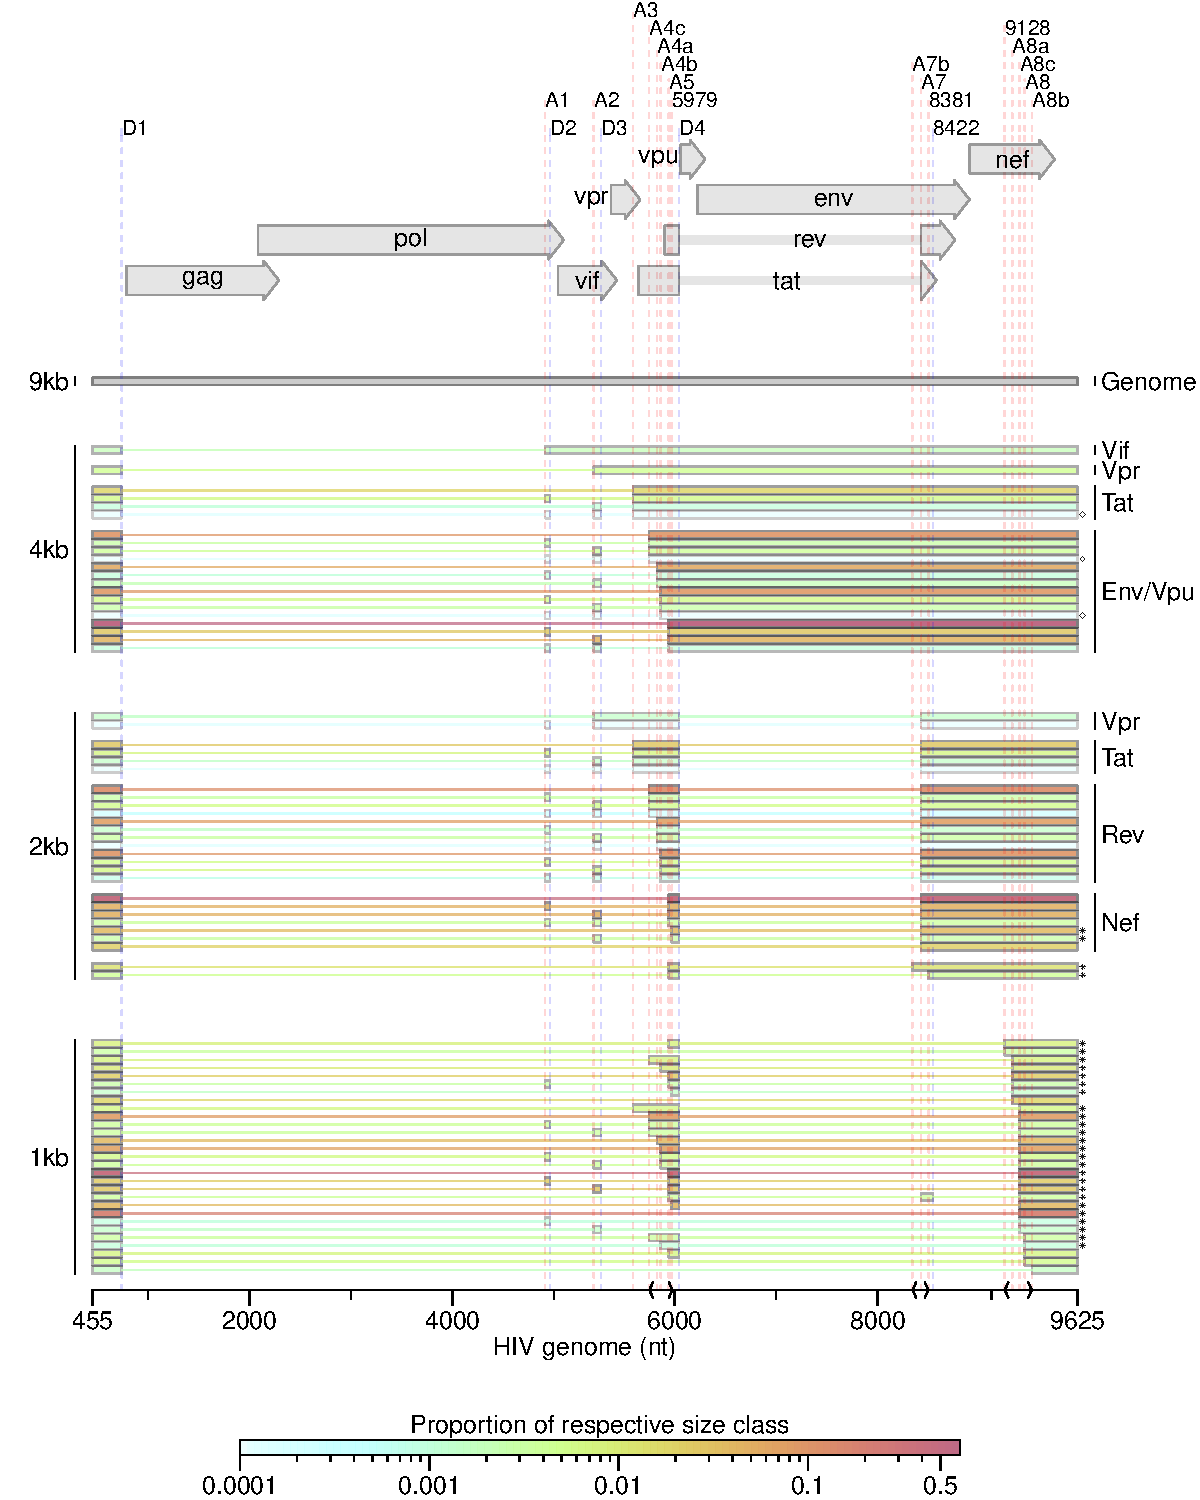
\includegraphics[width=.9\textwidth]{2.pdf}
	\caption[Spliced transcripts produced from \hivEight{}]{\hivEight{} transcripts in T cells for which the full message structure was determined are shown arranged by size class. Thick bars correspond to exons and thin lines to excised introns. For the well-conserved transcripts, encoded proteins are indicated. The relative abundance of each transcript within its size class is indicated by color. Asterisks denote transcripts that have not been reported previously to our knowledge. Of the 47 conserved HIV-1 transcripts, three were detected in fewer than five reads (indicated with $\diamond$) and two messages were not detected and are not shown (one encoding Vpr and one encoding Env/Vpu). Depicted non-conserved transcripts (using novel or cryptic splice sites) were each detected in at least five independent sequence reads across samples from at least two different human T-cell donors.}
	\label{figTranscripts}
\end{figure}

%[[italicize proteins]]
%[[SUPPLEMENTARY]]

Several groups have demonstrated tissue- and differentiation-specific splicing of cellular genes \citep{Wang2008,Grabowski2011,Llorian2011}. Importantly for HIV, these include changes during T-cell activation \citep{Ip2007,Topp2008}, raising the question of how cell-specific splicing affects HIV replication. While most studies of HIV-1 splicing have been conducted in cell lines using lab-adapted viral strains, limited works in PBMCs from infected patients, monocytes and macrophages have suggested that differences may indeed exist in relevant cell types \citep{Carrera2010,Saltarelli1996,Sonza2002,Dowling2008}. Moreover, human splicing patterns differ between individuals, but such polymorphisms have not been investigated in the context of HIV infection \citep{Hull2007,Kwan2007}.

For studies of transcript dynamics, reads from primer pairs 1.2, 1.3 and 1.4 containing junctions between D1 or any donor and each of five mutually exclusive acceptors, A3, A4c, A4a, A4b, A5 and A5a, were collected and their ratios calculated. 

\subsection{Statistical analysis}
Statistical modeling was performed using generalized linear modeling as described in Supplementary Report S2. All analyses were performed in R 2.14.0 (R Development Core) \citep{RCoreTeam2012}. 

\subsection{Data access}
Sequence data is available in the SRA database with the following accession numbers: SRP014319.

\section{Results}
\subsection{Sequencing HIV-1 transcripts produced in primary T cells and HOS cells}
In order to characterize HIV-1 transcript populations, we prepared viral cDNA from primary \cdFour{} T cells of seven different healthy human donors infected in vitro with \hivEight{}, an early passage dual-tropic clade-B clinical isolate (Supplementary Figure S1, human donor data in Supplementary Table S1) \citep{Collman1992}. We also studied HIV messages produced in infected HOS cells engineered to express CD4 and CCR5 (HOS-CD4-CCR5) because these cells support efficient HIV replication and engineered variants are widely used in HIV research. HOS cells were harvested at 18, 24 and 48 hours post infection (hpi) to investigate longitudinal changes during infection, and for comparison to 48 h infected T cells.

To preserve the relative proportions of template molecules while amplifying the cDNA, we used RainDance Technologies' single-molecule micro-droplet based PCR \citep{Tewhey2009}. Droplet libraries containing multiple overlapping primer pairs were designed to query all message forms and allow later calculation of relative abundance (Supplementary Table S2 and Supplementary Figure S1). Each primer was unique so that sequences could be assigned to a specific primer pair, which helped reconstruct the origin of sequence reads and deduce message structures. Amplified DNA products were sequenced using Single Molecule Real-Time (SMRT) technology from Pacific Biosciences \citep{Eid2009,Travers2010}. We obtained 847 492 filtered reads of amplified HIV-1 transcripts in primary \cdFour{} T cells and 89 350 in HOS cells. The longest sequenced continuous stretch of HIV-1 cDNA was 2629 bp. 


\subsection{Splice donors and acceptors}
We aligned PacBio reads containing HIV sequences to the \hivEight{} genome and identified candidate introns as recurring gaps in our sequences. Using this approach, we observed splicing at each of the widely conserved major splice donors and acceptors and several published cryptic sites (Figure \ref{figDonorAccept}A, hereafter referred to by their identifications shown in this figure, `D' for donors, `A' for acceptors).

In addition, we identified 13 putative novel splice sites: 2 donors and 11 acceptors (Figure \ref{figDonorAccept} and Supplementary Table S3). In order to be selected as a bona fide splice site and remove artifacts possibly created by recombination during sample preparation, we required that the new acceptor or donor was observed spliced to previously reported splice donors or acceptors in $>10$ sequence reads in \cdFour{} T cells. The most frequently used novel splice site was an acceptor that we have termed A8c because it lies near A8, A8a and A8b (discussed in detail below). Additional novel sites are further discussed in Supplementary Report S1.

Most of the new splice sites adhered to consensus sequences for the standard spliceosome (Supplementary Table S3). However, there appeared to be one splice donor upstream of D1 with a cytidine in place of the usual uracil 2 nt downstream of the splice site. Similar `GC donors' appear in 1\% of known splice junctions in humans \citep{Thanaraj2001}. Of the novel splice acceptors, three were preceded by dinucleotides other than the consensus AG. Alternative dinucleotides are used infrequently as splice acceptors \citep{Aebi1986,Burset2000,Burset2001,Sheth2006}; however, it is possible that our deep sequencing method allowed us to observe rare events. 


\subsection{Structures of spliced \hivEight{} RNAs}
To quantify the populations of HIV-1 transcripts, we aligned all reads to the collection of 47 well-established spliced HIV-1 transcripts and detected 45 of them (Figure \ref{figTranscripts}). We additionally aligned reads to the \hivEight{} genome allowing all possible combinations of splice junctions---canonical, cryptic or novel---determined from the sequencing data (Figure \ref{figDonorAccept}), yielding an additional 32 complete transcripts, 19 of which were novel. The data also provide evidence for more novel splice junctions but in incomplete sequences, implying the existence of additional new transcripts (Supplementary Table S4 and Supplementary Report S1). The full data set taken together provides evidence for least 109 different \hivEight{} transcripts in primary T cells.

Amplification primers that isolated the two main classes of spliced messages allowed us to determine the ratios of mRNAs in each (Figure \ref{figTranscripts} and Supplementary Table S5). Within the partially spliced class of transcripts, \textit{env}/\textit{vpu}, \textit{tat} (1-exon), \textit{vpr} and \textit{vif} messages existed in an average ratio of 96:4:$<1$:$<1$ in \cdFour{} T cells. The ratio of \textit{nef}:\textit{rev}:\textit{tat}:\textit{vpr} within the $\approximately{}2$ kb transcript class was 64:33:3:$<1$. Consistent with previous reports, the most abundant transcript in each class contained the splice junction from D1 to A5 (D1\^{}A5)---an \textit{env}/\textit{vpu} transcript contributing 64\% of the partially spliced class, and a completely spliced \textit{nef} transcript contributing 47\% of $\approximately{}2$ kb messages (Figure \ref{figTranscripts}) \citep{Purcell1993,Guatelli1990}. The relatively low abundance of transcripts encoding Tat suggests that Tat sufficiently stimulates HIV transcription elongation at low concentrations, or that the \textit{tat} transcripts must be efficiently translated. Due to biases inherent in the reverse transcription step, we could only compare transcripts within each size class, and we note that our methods have not been validated for empirical quantification. However, the ratios were roughly confirmed using overlapping sequence reads obtained with alternate primer pairs and by end point RT-PCR analysis of HIV-1 RNAs (data not shown).

Exons 2 and 3 are non-coding exons whose inclusion in transcripts other than \textit{vif} and \textit{vpr} has no known function. We found that they were included in other messages infrequently, each in $\approximately{}7$--8\% of transcripts in the $\approximately{}2$ kb completely spliced class of transcripts and 5\% of partially spliced transcripts accumulating in T cells. This is consistent with previous measurements in the partially spliced class but much lower than has been estimated for completely spliced transcripts in HeLa cells, suggesting cell-type-specific splicing patterns may influence inclusion of these exons \citep{Purcell1993}. 


\subsection{A novel $\approximately{}1$ kb class of completely spliced transcripts}
Primers placed near the \fivePrime{}- and \threePrime{}-ends of the \hivEight{} genome amplified a second class of completely spliced transcripts $\approximately{}1$ kb in length. In place of A7, these transcripts use a set of little studied splice acceptors located $\approximately{}800$ bp downstream within the \threePrime{}-TR. Two groups have previously observed splicing from D1 to acceptors A8, A8a and A8b in this region, yielding messages of this size class in patient samples; however, none of these could be translated to a protein of significant length \citep{Carrera2010,Smith1992}. We determined the complete structure of 29 members of the 1-kb class (Figure \ref{figTranscripts} and Supplementary Table S5). The most abundant messages observed in this class use the novel acceptor A8c to define their terminal exon. For HIV89.6, acceptor A8c was used nearly as frequently as A7, which gives us the 2-kb class of transcripts (Supplementary Table S3), and this was supported by end point RT-PCR analysis (data not shown).

Acceptor A8c is not well conserved in HIV-1/SIVcpz (14\%), although it is conserved in clade G viruses ($>95$\%) and most HIV-2/SIVsmm genomes (86\%) \citep{Kuiken2010}. This is due to the poor conservation of an adenosine at the wobble base position of the 123rd codon (proline) of the Nef reading frame, which creates the AG dinucleotide generally required at splice acceptors. Since any base at this position would code for proline, there does not seem to be strong selection for a splice acceptor here. However, A8c is displaced from nearby well-conserved ($>90$\%) cryptic acceptors A8a and A8b by multiples of 3 bp (12 and 21 bp, respectively), so splicing to any of these three acceptors would create similar ORFs. All HIVs and SIVs maintain at least one of these three acceptors, suggesting possible function \citep{Kuiken2010}. We confirmed that the 1 kb transcripts using A8a, A8b and A8c were present in infected HOS and T cells by end point RT-PCR using additional primer pairs and by Sanger sequencing of cloned transcripts (Figure \ref{figA8c}A and B; data not shown). 

\begin{figure}
	\centering
	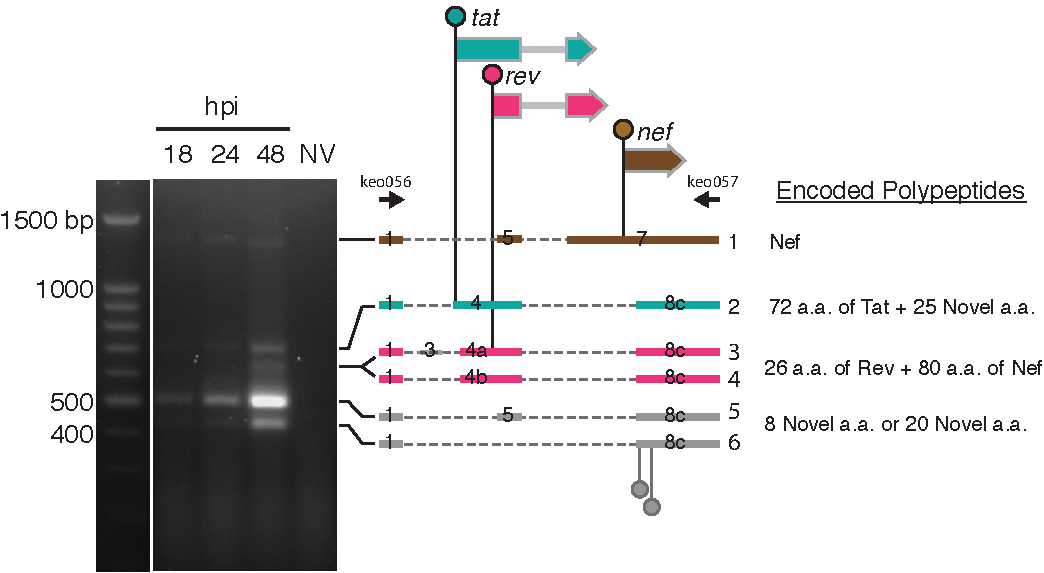
\includegraphics[width=.9\textwidth]{3.pdf}
	\caption[Novel transcripts utilizing acceptor A8c]{\hivEight{} transcripts were amplified by RT-PCR using RNA from infected HOS-CD4-CCR5 cells with primers keo056 and keo057. Major bands detected after gel electrophoresis were cloned from the 48 hpi sample and message structures determined by Sanger sequencing. Thick bars represent exons and dashed lines excised introns. Genes are shown above (not to scale) with start codons indicated by circles.  Messages 1, 2, 4 and 5 were cloned into expression plasmids for activity assays. (B) Confirmation of presence of the $\approximately{}1$ kb message RNAs in HOS-CD4-CCR5 and primary \cdFour{} T cells (human donor 1, harvested 24 and 48 hpi). An independent primer pair (keo058 and keo059) was used to amplify transcripts by RT-PCR. (C) Tat activity was measured in Tzm-bl cells as Tat-dependent luciferase production after transient transfection with expression plasmids. (D) Western blot showing expression of protein of the predicted size for Ref (12.5 kb) in cells transfected with the Ref expression construct and treated with proteasome inhibitor MG132, detected by an antibody recognizing the carboxy-terminus of Nef. Expression plasmid encoding Nef was included to control for possible expression of partial Nef peptides or breakdown products from the Nef ORF.}
	\label{figA8c}
\end{figure}

The 1-kb transcript containing exons 1, 4 and 8c (1-4-8c, where exon 8c begins at A8c and extends to the poly-adenylation site) encodes the first exon of Tat followed by 25 novel amino acids (termed Tat\^{}8c). Tat\^{}8c showed activity when overexpressed in cells containing a Tat reporter construct (Figure \ref{figA8c}C, nucleotide and amino acid sequences in Supplementary Table S6). Transcripts with exon structures 1-4a/b/c-8c encode a novel fusion of the amino-terminal 26 amino acids of Rev and the carboxy-terminal 80 amino acids of Nef, hereafter referred to as Ref. We did not detect Rev activity on overexpression of the \textit{ref} transcript, and Ref did not appear to interfere with the normal function of Rev or with HIV replication (Supplementary Figure S2). Ref was detectable by western blot using antibodies targeting the C terminus of Nef after inhibition of the proteasome, suggesting that the fusion is expressed but not stable (Figure \ref{figA8c}D). Thus, Ref has the potential to encode a new epitope potentially relevant in immune detection of HIV. The transcripts with exon structures 1-5-8c and 1-8c encode at most a short peptide, and so are candidates for acting as regulatory RNAs.

\subsection{Temporal dynamics of transcript populations}
To assess longitudinal variation, we investigated \hivEight{} transcript populations during the course of a single round of infection in HOS-CD4-CCR5 cells. A sensitive method for comparison among conditions involves quantifying utilization of six mutually exclusive splice acceptors A3, A4c, A4a, A4b, A5 and a novel acceptor just downstream of A5 termed A5a. Splicing at these acceptors determines the relative levels of messages encoding Tat and Env/Vpu in the partially spliced class and messages encoding Tat, Rev and Nef in the completely spliced class.

We observed longitudinal changes in the levels of these messages in HOS cells over 12--48 h that were statistically significant ($p < 10^{-10}$; generalized linear model described in Supplementary Report S2). This pattern was especially evident in junctions involving donor 1 spliced to each of these acceptors (Figure \ref{figJunctions}A). Most dramatically, transcripts with splicing junctions between D1 and A3 (tat messages) increased with time ($p < 10^{-10}$), while D1\^{}A4b junctions (used in \textit{env}/\textit{vpu} or \textit{rev} messages) were used reciprocally less ($p < 10^{-10}$). Such kinetic changes affecting specific transcripts both with and without the Rev-response element cannot be explained by the accumulation of Rev, and they may reflect differential transcript stability or HIV-induced alterations to the host splicing machinery. Temporal changes in HOS cells were confirmed using end point RT-PCR and analysis after electrophoresis on ethidium-stained gels (Figure \ref{figJunctions}B). 

\begin{figure}
	\centering
	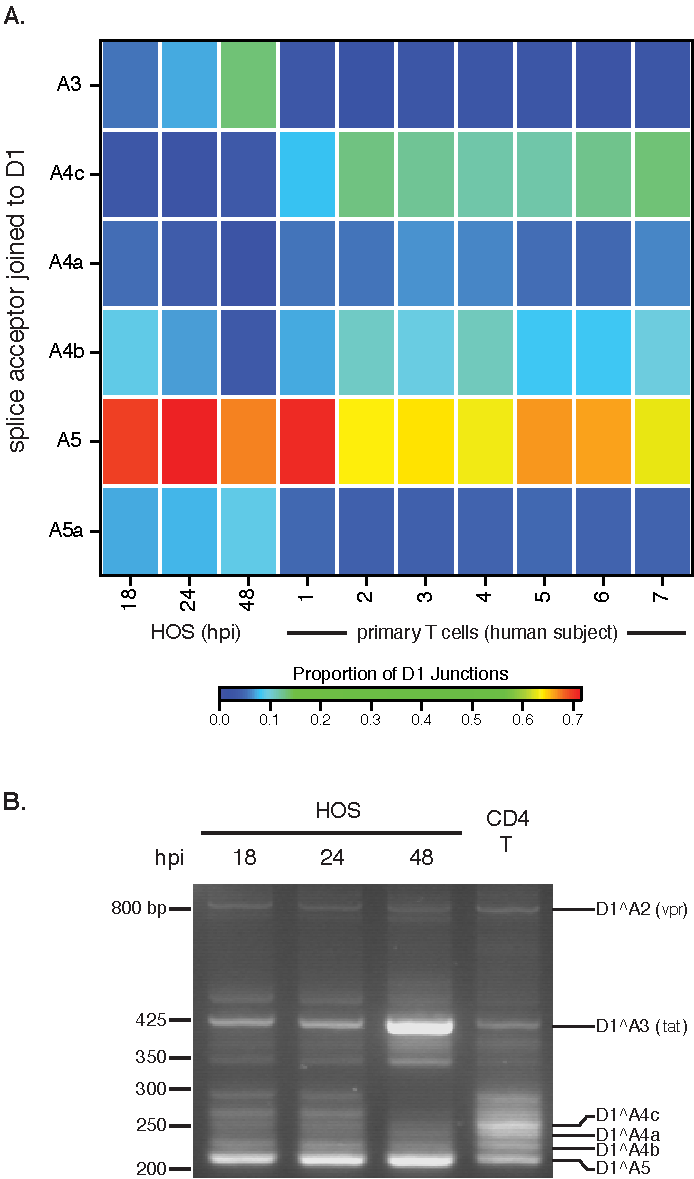
\includegraphics[width=.6\textwidth]{4.pdf}
	\caption[Temporal, cell type and donor variability in accumulation of HIV-1 messages]{Temporal, cell type and donor variability in accumulation of HIV-1 messages. (A) In order to highlight changes in ratios of HIV-1 transcripts accumulating over time during infection and between HOS-CD4-CCR5 cells and primary T cells, we used PacBio read counts to calculate proportions of transcripts with splicing from the first major splice donor, D1, to each of the mutually exclusive acceptors: A3, A4c, A4a, A4c, A5 and the novel putative acceptor A5a. The heat map shows average data for T cell and HOS cell samples in columns with the color tiles indicating the proportion of D1 splicing to each of the mutually exclusive acceptors (rows), according to the color scale shown. (B) Reverse transcription and bulk PCR amplification of \hivEight{} transcripts from HOS cells and primary T cells from one human subject (subject 3) resolved by agarose gel electrophoresis and stained with ethidium bromide verified temporal and cell type changes shown in (A).}
	\label{figJunctions}
\end{figure}

\subsection{Cell-type-specific splicing patterns}
We also compared splicing between T cells and HOS cells and found significant cell type differences ($p < 10^{-10}$). For example, while transcripts with D1\^{}A5 junctions were dominant in both cell types, messages using the D1\^{}A4c splice junction (encoding Env/Vpu or Rev) made up the bulk of the remaining transcripts in T cells but were a minor species in HOS-CD4-CCR5 cells. Likewise, Tat messages (using A3), which were quite abundant in HOS cells at all time points, contributed relatively little to populations of transcripts in primary T cells harvested at 48 hpi (Figure \ref{figJunctions}A). We also used end point PCR and analysis on ethidium-bromide-stained gels to confirm that the relative ratios of transcripts containing junctions to A3, A4a, A4b and A4c were different in HOS and T cells (Figure \ref{figJunctions}B).

\subsection{Human variation in HIV-1 splicing}

Quantitative comparisons also revealed modest differences in splicing between primary \cdFour{} T cells isolated from different human donors that were statistically significant ($p < 10^{-10}$) under a generalized linear model (Figure \ref{figJunctions}A). The magnitudes of predicted differences were small, all $<33$\% and most $<10$\%.


\section{Discussion}
Use of single-molecule enrichment and long-read single-molecule sequencing has made possible the most complete study to date of the composition of HIV-1 message populations, revealing several new layers of regulation. Studies of the low-passage HIV89.6 isolate in a relevant cell type showed numerous differences from studies of lab-adapted HIV strains in transformed cell lines, highlighting the importance of studying the most relevant models. These data also illustrate the limitations of gel-based assays for studying HIV-1 message population. Multiple different combinations of HIV-1 exons yield mRNAs of similar sizes that are easily confused in typical assays using gel electrophoresis. Thus, in many settings the more detailed information provided by single-molecule amplification and single-molecule DNA sequencing is more useful.

Using these methods, we have detected significant variations between HIV message populations generated in T cells from different human donors. The differences were modest compared to those observed between cell types or time points, perhaps not surprisingly since any human polymorphisms strongly affecting mRNA processing might interfere with normal gene expression. However, because tight calibration of message levels is important to HIV-1, the observed differences in message ratios might affect HIV-1 acquisition or disease progression. The variation in observed transcripts could also be affected by different kinetics of infection in T cells from the different donors. In either case, these data suggest that human polymorphisms may exist that affect HIV-1 message populations in infected individuals, providing a new candidate mechanism connecting human genetic variation with measures of HIV disease.

Sequences from the 89.6 viral strain revealed a class of small ($\approximately{}1$ kb) completely spliced transcripts, most contributed by splicing to a new poorly conserved acceptor A8c. These encoded two new proteins, one of which had Tat activity, and we showed that another, a Rev-Nef fusion termed Ref, could be detected in cells. \hivEight{} is a particularly cytotoxic virus isolated from the CSF of a patient, and it forms unusually large syncitia in macrophages \citep{Collman1992}. The abundance of 1-kb transcripts produced by this virus provides a possible explanation for its unique properties. In addition to the novel acceptor A8c, we have also identified 3 putative novel splice donors and 11 putative novel acceptors, which require further studied to clarify possible functions.

The wealth of new messages found here in \hivEight{} and in other HIV-1 isolates suggests there may be ongoing evolution of novel splice sites and new ORFs. Because splice acceptors in HIV-1 are weak \citep{Stoltzfus2009}, mutations creating sequences that even slightly resemble the \threePrime{} splice site consensus may be occasionally recruited as novel acceptors, creating new mRNAs. In fact, new splice signals may evolve with relative ease---it has been estimated that reasonable matches to the consensus for splice donors, acceptors and branch-point sites occur within random sequence every 290, 490 and 24 bp, respectively \citep{Burge1999}, though sequence substitutions in HIV are usually also constrained by overlapping viral coding regions. We and others have observed appearance of novel exons within the major HIV-1 introns \citep{Benko1990,Luetzelberger2006,Salfeld1990}. Such long stretches of RNA relatively devoid of competing splice sites may be particularly poised to evolve new signals. On the other hand, most of the putative novel splice acceptors we observed clustered near previously identified acceptors in HIV-1, suggesting that conserved cis-acting splicing signals may recruit factors that act promiscuously on new nearby sequences. Clusters of splice sites might also provide redundancies that protect vital messages, as suggested previously \citep{Abbink2008,Verhoef2001}. Frequent evolution of new splice sites may allow viruses to test out new combinations of exons, potentially yielding new RNAs and proteins, like those reported here. However, such novelty must compete with immune constraints---unstable novel polypeptides like Ref can be targeted to the proteasome and presented on MHC molecules as new epitopes for immune recognition.

HIV has likely evolved to produce calibrated message populations in T cells which seem to be altered with relative ease, as in infection in HOS cells, suggesting that therapeutic disruption of correct splicing may be feasible. A few studies have begun to explore small molecule therapy to disrupt HIV-1 splicing \citep{Bakkour2007,Tranell2011}. Several factors could be responsible for the differences we observed between HOS and T cells, including hnRNP A/B and H, SC35, SF2/ASF and SRp40 \citep{Caputi2004,Zahler2004}. Inhibition of SF2/ASF has already been shown to abrogate HIV-1 replication in vitro \citep{Bakkour2007}. Thus the lability seen here for function of these factors suggests they may be attractive antiretroviral targets. 

\section{Acknowledgements}
We would like to thank the University of Pennsylvania Center for AIDS Research (CFAR) for preparation of viral stocks and isolation of primary \cdFour{} T cells; James A. Hoxie, Ronald G. Collman, Jianxin You, Robert W. Doms, Paul Bates, David Rekosh and members of the Bushman laboratory for reagents, helpful discussion and technical expertise. F.D.B., K.T., D.L., E.S., K.E.O. and R.M. conceived and designed the experiment. K.E.O. and R.C.A. carried out sample preparation and experimental validation. P.D. and J.O. performed single-molecule amplification. K.T. and S.W. performed sequencing. S.S.-M., K.E.O. and M.B. analyzed the data. K.E.O., F.D.B. and S.S.-M. wrote the manuscript. 



\end{document}
